\chapter{Introduction}
  % TODO: A general introduction
  \lettrine[lines=2]{R}einforcement learning has demonstrated itself as one of the most promising
  branch of machine learning especially in the recent years.\newline
  RL success is mostly due to its applicability in large and complex control
  problem (robotics, economics, AI and so on) where the high complexity of the models
  involved makes impossible, for the human designer, to design a complete and
  efficient model.
  In all these different fields RL techniques are able to provide a sufficiently
  accurate estimation of the model dynamics.\newline
  A generic RL algorithm  permits an agent to \textit{learn} a specific
  \textit{task} by rewarding the agent when, during the training, it performs an
  action that brings it near to the goal or by punishing it when the action chosen
  bring it away from the goal (as described in Figure \ref{fig:rl-schema}).\newline

  \begin{figure}
    \centering
    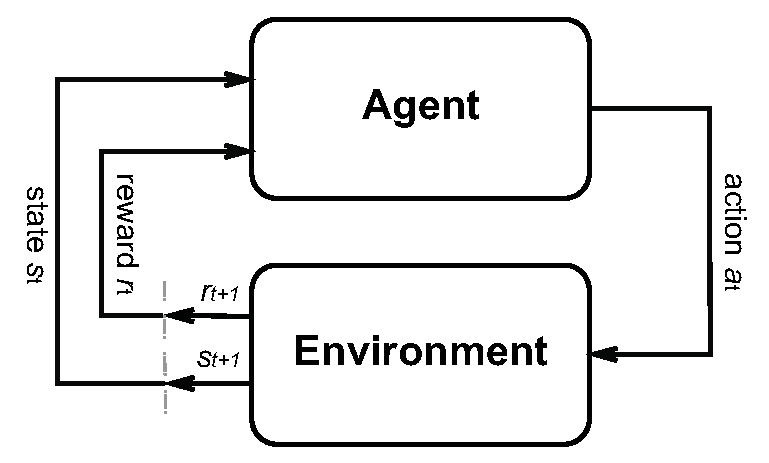
\includegraphics[scale=0.5]{images/rldiagram.eps}
    \caption{Schematization of the agent/environment interaction in RL}
    \label{fig:rl-schema}
  \end{figure}

  \noindent Many techniques exist to model such types of situations, one of the most popular
  and studied are the Markov Decision Processes (abbreviated as MDP). This formalism
  (we will give a more precise definition in chapter 2) permits to model the
  problem as a collection of states and actions. Besides a reward function is
  also defined and used by the agent during the training phase.\newline
  When both the model of the problem, that is when the probability distribution
  given a state-action pair is known to the designer of the problem, and when
  the reward function is known, well established and efficient techniques
  are available to optimally solve the problem (eg. Dynamic programming).\newline

  \noindent Unfortunately in many real-world situations the model and the reward function
  associated to the MDP are not known and need to be learned by the agent(\textit{model-free}).
  In this context the term \textit{"solving the problem"} acquires an additional meaning:
  we want still to determine the optimal policy but at the same time we want also
  learn the dynamics and reward function of the task. Some techniques do not even
  need to learn an explicit representation of reward and transition models but
  just need an intrinsic schematization of them. For example, Q-Learning (or
  Fitted algorithms) build at each iteration a representation of the Q function
  of the problem without building an explit representation of rewards and dynamics.

  \noindent A big problem in the model-free approach is the enormous amount of
  samples required to learn a good policy, this is true especially in many real world situation where
  the agent has a limited amount of time and resources to spend on the learning phase. Moreover every time the
  task at hand changes the entire learning process must be restarted from scratch even
  if very similar tasks have been already solved by the agent.\newline
  This problem motivates the need to have the possibility to transfer and reuse knowledge across
  different tasks. This idea naturally arises from psychology and cognitive science research (early 90s) where
  humans are shown to learn a specific task better and faster if they have already solved similar tasks in the past.\newline
  In the general machine learning framework the idea of the transfer of knowledge has already been successfully
  applied to problems in supervised learning (such as recommender systems, text classification, speech classification, etc.).\newline
  In the last 10 years the research on transfer learning has started to focus also on reinforcement learning applications.\newline
  In the RL field the main idea is that if the agent already knows the solution of a set of \textit{source tasks}, it
  can reuse that knowledge to speed up the learning of a new tasks (ie. the \textit{target task}).\newline
  Every transfer RL algorithm must answer two questions: \textit{what} and \textit{when} to transfer?\newline
  The first question can be answered in different ways: one possibility is to transfer instance of
  knowledge(ie. samples) from the source MDPs to the target MDP (\cite{lazaric2008transfer}), another possibility is
  representation transfer where the transfer algorithm changes the representation of the solution of the
  source tasks (\cite{singh2004intrinsically}), finally we have the possibility offered by parameters transfer where what we transfer
  is an initialization for the parameters of the learning algorithm of the target task (refer to \cite{lazaric2012transfer}).\newline
  This work focuses on the transfer of instances.\newline
  The second question highlights a very important point: if we focus on the transfer of samples between tasks, the
  transfer should only occur when the source task presents some similarities with respect
  to the target task, if not a phenomena, known in literature as \textit{negative transfer}, may occur.
  Negative transfer might actually worsen the performance of the learning algorithm over
  the target task and therefore must be avoided as much as possible(a possible solution is
  presented in \cite{lazaric2008transfer}, besides the problem will be deeply discussed in this thesis).\newline

  \noindent When considering the problem of the transfer of knowledge across multiple tasks, a series of natural
  questions must be answered: Where to fetch the next sample? From which task? Should it be fetched from
  a source task or directly from the target task?. Methods have been proposed in the past, such has \cite{lazaric2008transfer},
  where the authors introduce an algorithm which estimates the similarity between source and target tasks and selectively transfers
  from the source tasks which are more likely to provide samples similar to those generated by the target task.\newline
  Indeed many times the actual environment in which the agent lives is expensive, time-consuming and sometimes
  dangerous. The prohibitive cost of collecting samples in the real environment(ie. the target task)
  makes difficult (sometimes impossible) to learn a good policy, again this motivates the need for
  the reuse of knowledge.\newline

  \noindent Our approach differs from previous works: we try to perform transfer learning exploiting a very well known
  idea of statistics: importance sampling. All the samples are transferred to the target task but each sample is
  enriched with some information that permits the learning algorithm to correct the bias introduced inside the target.\newline
  More precisely we will propose an extension of well studied learning algorithm (Fitted Q-Iteration) to permit
  the reuse of experience samples. The algorithm, called \textbf{W}eighted \textbf{F}itted \textbf{Q-I}teration (from now on abbreviated as WFQI),
  tries to build an high level representation of reward and transition model of the task at hand and produces an
  estimation of the relevance (under the form of a weight) of the source samples with respect the target task. The
  resulting weights are then used, along with the source/target samples, in FQI with a weighted regression algorithm
  to build an accurate estimation of the Q function.\newline
  It is always important to remember that samples from the source tasks are cheap but they may negatively \textit{bias} the agent
  in the target tasks(ie. negative transfer), on the other hand samples coming from
  the target task are expansive(they require the agent to perform trajectories over the real environment)
  but are unbiased since they come from the same problem the agent is trying to solve.

  \section{Mission and Contributions}
    \noindent The mission of this thesis is to produce a novel method to exploit the reuse
    of knowledge in the solution of new tasks. This is done by modifying the standard
    Fitted Q-Iteration algorithm to permit the transfer of samples.
    We seek for the optimal tradeoff between the number of samples coming from the
    source tasks and the number of samples coming from the target task by
    controlling the amount of bias introduced in the target task versus
    the reduction in variance brought by the transferred samples.\newline
    Finally we try to prove a series of theoretical results over the performance
    of the above mentioned algorithm.\newline

    The contributions of this thesis can be summarized as follows:
    \begin{itemize}
      \item \textbf{Algorithmical} contribution: We introduce a modification
            of the standard Fitted Q-Iteration algorithm (WFQI) that
            makes possible the transfer of knowledge across multiple
            source tasks and we empirically demonstrate the performance

      \item \textbf{Theoretical} contribution: We develop a theoretical analysis of
            the Weighted Fitted Q-Iteration (WFQI) to understand performance and limitations
            of such algorithm.
    \end{itemize}

  \section{Contents Outline}
    \noindent This thesis is structured as follows:
    \begin{itemize}
      \item \textbf{Chapter 2} formally introduces the reader to the concept of
            Markov Decision Process and its application to reinforcement learning
            problems. In this chapter we introduce part of the notation that will
            be used in the rest of the thesis.
      \item \textbf{Chapter 3} provides an overview over the transfer learning
            framework including all the necessary mathematical notation. A short
            summary over the principal related works is included. This chapter also introduces the Fitted Q-Iteration algorithm.
      \item \textbf{Chapter 4} presents the idea behind importance sampling and formally introduce the framework
            to permit the transfer of knowledge. Additionally we proposes a modification of the standard FQI algorithm to
            allow the use of transferred samples.
      \item \textbf{Chapter 5} theoretically validates and motivates the proposed approach.
      \item \textbf{Chapter 6} provides and validates the performances of the algorithm
            described in the previous chapter.
      \item \textbf{Chapter 7} draws the conclusions and proposes some future line of work.
      \item \textbf{Appendix A} provides some additional details regarding the implementation of WFQI.
      \item \textbf{Appendix B} provides a theoretical background for Gaussian Process introducing the main
            theoretical and practical results of interest for this thesis.
    \end{itemize}
